\section{Combinar}
Este filtro consiste en cambiar la distribución de píxeles de una imagen tal que queden ordenados en cuatro cuadrantes diferentes. Se obtendrá mediante la aplicación de este filtro cuatro imágenes distintas de menor tamaño a la original, pero en donde los píxeles de la original se encuentran aun presentes en la imagen resultante. Es decir : 
\begin{center}
$\forall$ $pixel,$ $cantidadPixeles(pixel, imagenOriginal) == cantidadPixeles(pixel,imagenResultante)$ 
$\wedge$ $imagenOriginal.length == imagenResultante.length$ 
\end{center}
\begin{flushright}
 $pixel \in imagenOriginal$
\end{flushright}

El resultado visual que provoca la aplicación de este filtro es la sensación de que la imagen se dividió en cuatro pequeñas imágenes cuando verdaderamente ninguna de ella es igual a la otra. 
Se puede ver en el ejemplo de la figura 1 como es la distribución que va teniendo la aplicación de nuestro filtro allí podemos distinguir que los píxeles antes y luego de la aplicación del filtro son los mismos.
\begin{figure}[H]
\begin{subfigure}[b]{0.27\textwidth}   
\centering         
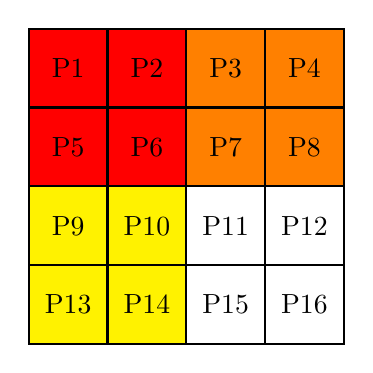
\begin{tikzpicture}
    [%%%%%%%%%%%%%%%%%%%%%%%%%%%%%%
        box/.style={rectangle,draw=black,thick, minimum size=1cm},
    ]%%%%%%%%%%%%%%%%%%%%%%%%%%%%%%
\draw[step=1cm,color=gray] (-2,-2) grid (2,2);
\node[box, fill=red] at (-1.5,+1.50) {P1};
\node[box, fill=red] at (-0.50,+1.50) {P2};
\node[box, fill=orange] at (+0.50,+1.50) {P3};
\node[box, fill=orange] at (+1.5,+1.50) {P4};
\node[box, fill=red] at (-1.5,+0.50) {P5};
\node[box, fill=red] at (-0.50,+0.50) {P6};
\node[box, fill=orange] at (+0.50,+0.50) {P7};
\node[box, fill=orange] at (+1.50,+0.50) {P8};
\node[box, fill=yellow] at (-1.50,-0.50) {P9};
\node[box, fill=yellow] at (-0.50,-0.50) {P10};
\node[box] at (+0.50,-0.50) {P11};
\node[box] at (+1.50,-0.50) {P12};
\node[box, fill=yellow] at (-1.50,-1.50) {P13};
\node[box, fill=yellow] at (-0.50,-1.50) {P14};
\node[box] at (+0.50,-1.50) {P15};
\node[box] at (+1.50,-1.50) {P16};
\end{tikzpicture}
\end{subfigure}
{\LARGE$\xrightarrow{TRANSFORMACION}$}
\begin{subfigure}[b]{0.27\textwidth} 
\centering           
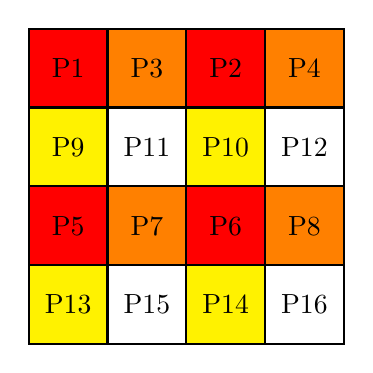
\begin{tikzpicture}
    [%%%%%%%%%%%%%%%%%%%%%%%%%%%%%%
        box/.style={rectangle,draw=black,thick, minimum size=1cm},
    ]%%%%%%%%%%%%%%%%%%%%%%%%%%%%%%
\draw[step=1cm,color=gray] (-2,-2) grid (2,2);
\node[box, fill=red] at (-1.5,+1.50) {P1};
\node[box, fill=orange] at (-0.50,+1.50) {P3};
\node[box, fill=red] at (+0.50,+1.50) {P2};
\node[box, fill=orange] at (+1.5,+1.50) {P4};
\node[box, fill=yellow] at (-1.5,+0.50) {P9};
\node[box] at (-0.50,+0.50) {P11};
\node[box, fill=yellow] at (+0.50,+0.50) {P10};
\node[box] at (+1.50,+0.50) {P12};

\node[box, fill=red] at (-1.50,-0.50) {P5};
\node[box, fill=orange] at (-0.50,-0.50) {P7};
\node[box, fill=red] at (+0.50,-0.50) {P6};
\node[box, fill=orange] at (+1.50,-0.50) {P8};

\node[box, fill=yellow] at (-1.50,-1.50) {P13};
\node[box] at (-0.50,-1.50) {P15};
\node[box, fill=yellow] at (+0.50,-1.50) {P14};
\node[box] at (+1.50,-1.50) {P16};
\end{tikzpicture}
\end{subfigure}
\caption{Distribución de píxeles tras aplicar el filtro de combinar}
\end{figure}

También podemos ver en la figura 2 cual es el impacto de nuestro filtro en una imagen real, podremos notar aquí lo parecidas que son imágenes resultantes en cada uno de los cuadrantes, a nuestro ojo es casi imperceptible la diferencia.

\begin{figure}[H]
\begin{subfigure}[b]{0.50\textwidth} 
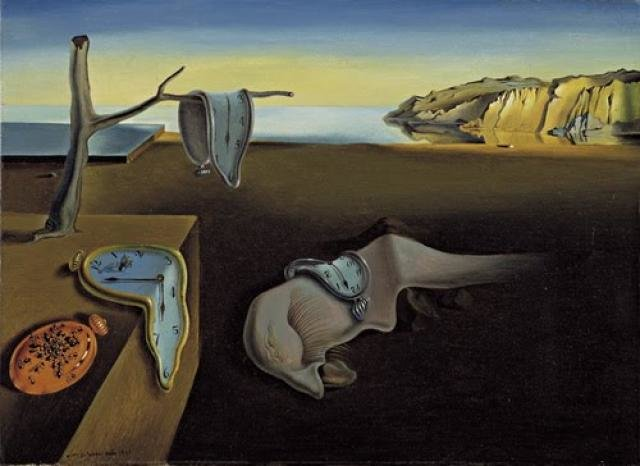
\includegraphics[scale=0.4]{img/fourCombine_before.jpg}
\end{subfigure}
{\LARGE$\xrightarrow{T}$}
\begin{subfigure}[b]{0.50\textwidth} 
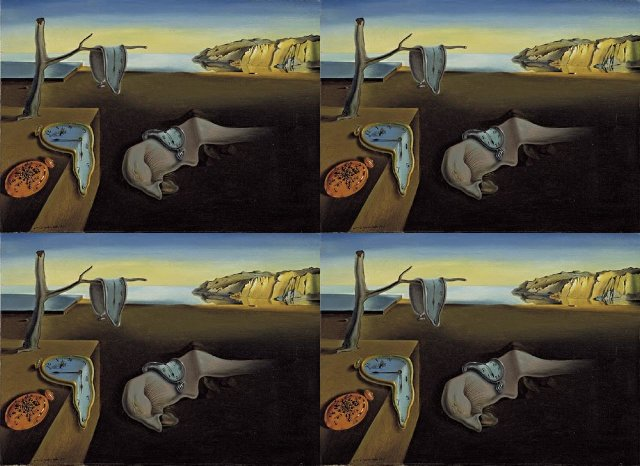
\includegraphics[scale=0.4]{img/fourCombine_after.jpg}
\end{subfigure}

\caption{Imagen real antes y luego de la aplicación del filtro}
\end{figure}

\subsection{Implementación}
\subsubsection*{Explicación general de la solución}
\paragraph{Solución en código C}
La solución que fue planteada en c consiste en recorrer la matriz asociada a la imagen de entrada una sola vez píxel por píxel. Cada uno de estos píxeles posee una coordenada y por medio de esta se calcula la coordenada en la matriz asociada a la imagen de salida. 


\paragraph{Solución en ASM}
En cuanto a la implementación en código assembler se tuvo que pensar una solución totalmente diferente ya que al tener que hacerlo con registros de 128 bits nuestra solución de agarrar los píxeles uno por uno y calcular su lugar correspondiente no seria posible. Se tomaron las siguientes decisiones de modelado Decisiones de modelado:
\begin{itemize}
\item Decidir con cuanta información a la vez íbamos a trabajar , se llego a la conclusión que lo mejor seria trabajar con 8 píxeles a la vez. Esta decisión se tomo puesto que eligiendo los 8 píxeles del lugar correcto podíamos llegar a armar 8 píxeles que iban a ser puestos en la imagen de salida. Esto nos debería dar un ahorro en la cantidad de veces que vamos a pegarle a memoria.
\item Decidir entre la posibilidad de agarrar 16 píxeles que este en la misma fila o que estén la misma columna. Nos pareció lo mas fácil de implementar y lo mas efectivo a la hora de usar la cache era que tomáramos 8 píxeles contiguos. Se vera mas adelante en un experimento la diferencia entre ambos
\item Ya que íbamos a tomar de a 8 píxeles contiguos pero el enunciado del trabajo practico solo aseguraba que la imagen a lo ancho iba a ser múltiplo de 4 , teníamos que hacer algo con respecto a los casos donde la imagen no era múltiplo de 8. En este caso tratamos de emular un poco la practica que realiza muchas veces el compilador de intel donde este separa el código en casos especiales para poder ahorrarse de preguntar en el medio del código . Por ende en nuestro código ASM solo preguntamos una vez si el ancho es múltiplo de 4 o de 8 y dependiendo de eso el código se disfurca en dos
\end{itemize}

Ahora hablemos un poco mas de la iteración dentro del un ciclo de nuestro código ASM , podemos separar lo que hace dentro de una columna de lo que hace al cambiar de fila. Dentro de una columna nuestro objetivo es agarrar 8 píxeles llámense $Pi$ con $1\leq i\leq 8$ y trabajarlos de forma tal que queden listos para ser pegados en la memoria de la imagen destino. El siguiente gráfico nos mostrara como ocurre la transformación de los 8 píxeles desde que son extraídos desde la imagen fuente hasta que están listos para ser puestos en la imagen destino : 

\begin{tikzpicture}
\matrix [matrix of nodes,row sep=,row sep=0mm,
column 1/.style={nodes={rectangle,draw,minimum width=3em}},
column 2/.style={nodes={rectangle,draw,minimum width=3em}},
column 3/.style={nodes={rectangle,draw,minimum width=3em}},
column 4/.style={nodes={rectangle,draw,minimum width=3em}},
] (P)
{
P8 & P7 & P6 & P5\\
};
\end{tikzpicture}
\begin{tikzpicture}
\matrix [matrix of nodes,row sep=,row sep=0mm,
column 1/.style={nodes={rectangle,draw,minimum width=3em}},
column 2/.style={nodes={rectangle,draw,minimum width=3em}},
column 3/.style={nodes={rectangle,draw,minimum width=3em}},
column 4/.style={nodes={rectangle,draw,minimum width=3em}},
] (P)
{
P4 & P3 & P2 & P1\\
};
\end{tikzpicture}


Separo en pares e impares

\begin{tikzpicture}
\matrix [matrix of nodes,row sep=,row sep=0mm,
column 1/.style={nodes={rectangle,draw,minimum width=3em}},
column 2/.style={nodes={rectangle,draw,minimum width=3em}},
column 3/.style={nodes={rectangle,draw,minimum width=3em}},
column 4/.style={nodes={rectangle,draw,minimum width=3em}},
] (P)
{
0 & P7 & 0 & P5\\
};
\end{tikzpicture}
\begin{tikzpicture}
\matrix [matrix of nodes,row sep=,row sep=0mm,
column 1/.style={nodes={rectangle,draw,minimum width=3em}},
column 2/.style={nodes={rectangle,draw,minimum width=3em}},
column 3/.style={nodes={rectangle,draw,minimum width=3em}},
column 4/.style={nodes={rectangle,draw,minimum width=3em}},
] (P)
{
0 & P3 & 0 & P1\\
};
\end{tikzpicture}

\begin{tikzpicture}
\matrix [matrix of nodes,row sep=,row sep=0mm,
column 1/.style={nodes={rectangle,draw,minimum width=3em}},
column 2/.style={nodes={rectangle,draw,minimum width=3em}},
column 3/.style={nodes={rectangle,draw,minimum width=3em}},
column 4/.style={nodes={rectangle,draw,minimum width=3em}},
] (P)
{
P8 & 0 & P6 & 0\\
};
\end{tikzpicture}
\begin{tikzpicture}
\matrix [matrix of nodes,row sep=,row sep=0mm,
column 1/.style={nodes={rectangle,draw,minimum width=3em}},
column 2/.style={nodes={rectangle,draw,minimum width=3em}},
column 3/.style={nodes={rectangle,draw,minimum width=3em}},
column 4/.style={nodes={rectangle,draw,minimum width=3em}},
] (P)
{
P4 & 0 & P2 & 0\\
};
\end{tikzpicture}


Shifteo pre juntar

\begin{tikzpicture}
\matrix [matrix of nodes,row sep=,row sep=0mm,
column 1/.style={nodes={rectangle,draw,minimum width=3em}},
column 2/.style={nodes={rectangle,draw,minimum width=3em}},
column 3/.style={nodes={rectangle,draw,minimum width=3em}},
column 4/.style={nodes={rectangle,draw,minimum width=3em}},
] (P)
{
P7 & 0 & P5 & 0\\
};
\end{tikzpicture}
\begin{tikzpicture}
\matrix [matrix of nodes,row sep=,row sep=0mm,
column 1/.style={nodes={rectangle,draw,minimum width=3em}},
column 2/.style={nodes={rectangle,draw,minimum width=3em}},
column 3/.style={nodes={rectangle,draw,minimum width=3em}},
column 4/.style={nodes={rectangle,draw,minimum width=3em}},
] (P)
{
0 & P4 & 0 & P2\\
};
\end{tikzpicture}

Los uno cruzados con un or

\begin{tikzpicture}
\matrix [matrix of nodes,row sep=,row sep=0mm,
column 1/.style={nodes={rectangle,draw,minimum width=3em}},
column 2/.style={nodes={rectangle,draw,minimum width=3em}},
column 3/.style={nodes={rectangle,draw,minimum width=3em}},
column 4/.style={nodes={rectangle,draw,minimum width=3em}},
] (P)
{
P7 & P3 & P5 & P1\\
};
\end{tikzpicture}
\begin{tikzpicture}
\matrix [matrix of nodes,row sep=,row sep=0mm,
column 1/.style={nodes={rectangle,draw,minimum width=3em}},
column 2/.style={nodes={rectangle,draw,minimum width=3em}},
column 3/.style={nodes={rectangle,draw,minimum width=3em}},
column 4/.style={nodes={rectangle,draw,minimum width=3em}},
] (P)
{
P8 & P4 & P6 & P2\\
};
\end{tikzpicture}

Hago shuffle 

\begin{tikzpicture}
\matrix [matrix of nodes,row sep=,row sep=0mm,
column 1/.style={nodes={rectangle,draw,minimum width=3em}},
column 2/.style={nodes={rectangle,draw,minimum width=3em}},
column 3/.style={nodes={rectangle,draw,minimum width=3em}},
column 4/.style={nodes={rectangle,draw,minimum width=3em}},
] (P)
{
P7 & P5 & P3 & P1\\
};
\end{tikzpicture}
\begin{tikzpicture}
\matrix [matrix of nodes,row sep=,row sep=0mm,
column 1/.style={nodes={rectangle,draw,minimum width=3em}},
column 2/.style={nodes={rectangle,draw,minimum width=3em}},
column 3/.style={nodes={rectangle,draw,minimum width=3em}},
column 4/.style={nodes={rectangle,draw,minimum width=3em}},
] (P)
{
P8 & P6 & P4 & P2\\
};
\end{tikzpicture}


Una vez que tenemos los 8 píxeles ordenados según los quiero procedo a guardarlos en la posiciones de memoria a las que apuntan el registro $R8$ y $R9$ sin preocuparme en este caso del cuadrante donde estos dos están apuntando.

En cuando a que pasa cuando la iteración sobre la columna se termina y se pasa a una nueva columna lo vamos a explicar a continuación:
Primero movemos $R8$ y $R9$ hacia su próxima fila recordando que la próxima fila sea cual sea el cuadrante donde se encuentro se realiza sumándole una fila a cada uno.

El tema viene ahora en que hay que ir switcheando los cuadrantes donde voy insertando los píxeles resultantes cada uno fila. Siendo esta parte del código la que se encarga de swtichear $R8$ y $R9$ entre los distintos cuadrantes se utiliza para ello una variable puente para no sobrescribir ni pisar ningún valor. 

Snippet del código :

\begin{lstlisting}
		mov rax, r8
		mov r8, r10
		mov r10, rax
		mov rax, r9
		mov r9, r11
		mov r11, rax
\end{lstlisting}

Lo único que cambia de esta explicación con respecto a cuando el ancho no es multiplico de 8 es en este punto donde tenemos que cambiar de fila, ya que nos quedaron 4 píxeles sin procesar y como seria demasiado trabajoso holdearlos para poder trabajarlos en otra iteración posterior, lo mejor que nos ocurrió fue trabajarlos manualmente e insertarlos en el lugar donde les corresponde. Luego de esto se sigue con el paso recién explicado.


\subsection{Análisis preliminar}
\subsubsection*{Comparar para distintos tamaños, relaciones entre implementaciones}
\begin{figure}[H]
\centering
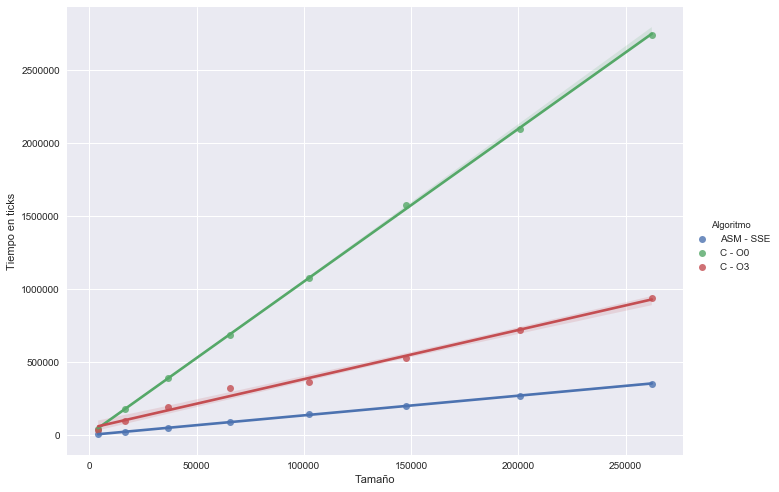
\includegraphics[scale=0.5]{img/fourCombine_CvsASMvsO3.png}
\caption{Comparación llana de las implementaciones en C contra la implementación en ASM}
\label{sec:ticksciclo}
\end{figure}
\subsubsection*{Comparación de rendimiento de ASM vs C}
Luego de sacar manualmente un poco del ruido podemos ver una clara diferencia entre la implementación de C y la de ASM. Dato curioso que podemos agregar entre la diferencia de O0 y O3 es que al momento de compilar con gcc ( gracias a la herramienta \url{https://godbolt.org/} ) se puede apreciar como una linea de código se vuelve ASM dependiendo el flag. 

Después de analizarlo los resultados tanto en O0 como en O3 podemos ver que esta linea de código :

\begin{lstlisting}
		mDst[offsetH + (h >> 1)][offsetW + (w >> 1)] = mSrc[h][w];
\end{lstlisting}

Cuando se encuentra el flag de O0 activado $h >> 1$ se calcula todas las veces, en cambio cuando el flag de O3 esta activo esto no sucede y se calcula antes de ciclar. Existen otras mejoras pero el nivel del código no nos permitió encontrarlas. Nos pareció interesante en este gráfico dejar todos tiempos que fuimos midiendo para ver que tal se comporta el ordenador cuando medimos tiempos aunque hay un poco de outliners la gran mayoría de los tiempos rondan en lo mismo.

\subsection{Hipótesis de trabajo}
\subsubsection*{Conjunto de ideas de experimentos}
Una de las primeras ideas a la hora de experimentar con nuestra implementación de ASM es poder correrla en contra de la de implementación que se realizo en C , teniendo en cuenta que en el caso de este filtro juega mas el echo de guardar en memoria los datos que de procesarlos.

También tratamos de llevar a cabo en este conjunto de experimentación la idea de Loop unrolling , con alguna pequeña modificación. Si vamos a lo que se entiende como Loop unrolling y lo aplicamos al algoritmo de ASM lo que lograríamos seria leer de a 16 píxeles a lo largo a la vez en de a 8 píxeles logrando así una reducción en los saltos del loop de columna. Pero esta implementación nos llevaría a tener que abrir mas los casos en los cuales anteriormente tratábamos ahora tendríamos imágenes que deberían ser congruentes a 0 modulo 16 para poder ir por el camino del unrolling pero caso contrario es decir ser congruente 4, 8 , 12 deberían tratarse en otra parte del programa y así solo logrando un incremento en la performance para 0.25 de los casos. Para poder solventar este pequeño numero de casos donde el unrolling podría ser efectivo se decidió procesar 16 píxeles a la vez pero distribuidos en dos filas , de esta manera solo habría que tener en cuenta que las filas sean múltiplos de 2 es decir pares para poder aplicar esta mejora al algoritmo.

Otra idea que había surgido para probar en un experimento fue la de usar registros mas grandes (AVX) para poder lograr así una reducción a la hora de mezclar los elementos, se había pensado que teniendo muchos mas píxeles juntos iba a resultar mas fácil poder ordenarlos para su posterior puesta en en memoria. El problema con este experimento fue que encontramos que las instrucciones AVX (que funcionan en 256 bits) lo único que hacen es replicar comportamientos en la parte baja y la alta del registro es decir los trata como dos registros de 128 bits que solo logran comportamientos de este tipo de registro. Desistimos de hacer este experimento por no encontrar las instrucciones necesarias para poder realizar un código mas performante que el propuesto como solución. 
\subsubsection*{Afirmaciones que buscan probar verdaderas}
Buscamos mediante distintos sistemas de medidas mostrar que desenrollar el loop aumenta la performance de nuestro algoritmo ya que el sistema de predicción debería predecir menos saltos.

\subsection{Diseño experimental}
\subsubsection*{Explicación de como y que van a medir}
Queremos ver bien de cerca que es lo que pasa con nuestras dos implementaciones porque si tomamos las medidas en una escala muy chica vamos a perder información sobre que lo que esta pasando. 

También nos gustaría saber cual es el tiempo que se demoran ambos algoritmos en desarrollar un ciclo. Sabemos que la diferencia esta en que ambos resuelven diferente cantidad de  píxeles a la vez, por ende el tiempo que demoren en resolver un ciclo va a estar dividido por la cantidad de elementos que trabaja a la vez. Vamos a poner también en la misma linea el tiempo de un ciclo del algoritmo de c que solo procesa un píxel a la vez.

Un experimento interesante que debería estar incluido en el tp sería poder medir que porcentaje de un ciclo del algoritmo presentado como respuesta se utiliza cargando datos, que porcentaje en procesarlos y que porcentaje en cargarlos nuevamente a memoria, tenemos la impresión que la gran mayoría del tiempo se la pasa cargando y poniendo cosas en memoria por ende si quisiéramos mejorar aun mas nuestro algoritmo podríamos solamente trabajar sobre el porcentaje de procesamiento de los datos. Estaríamos en presencia de un cuello de botella representado por la memoria.

El roll del cache en imágenes grandes aquí vamos a probar cual es la diferencia entre la implementación presentada como respuesta al trabajo practico y la implementación del unrolling. Aunque anteriormente vimos que en ejemplos chicos la implementación del unrolling era mejor, en el caso de imágenes obscenamente grandes (mayores a la capacidad del cache) esto no ocurre en imágenes grandes.
\subsubsection*{Explicación del conjunto de datos de entrada}
En el único momento que vamos a utilizar datos por fuera de la cátedra va a ser al momento de querer ver el funcionamiento de la cache en nuestro algoritmo, en este caso utilizamos una imagen que excede la cache de nuestra CPU , la imagen pesa 200mb y por obvios motivos no va a ser adjuntada junto al tp.
\subsection{Resultados y Análisis}
\subsubsection*{Resultados obtenidos, gráficos y tablas}
\begin{figure}[H]
\centering
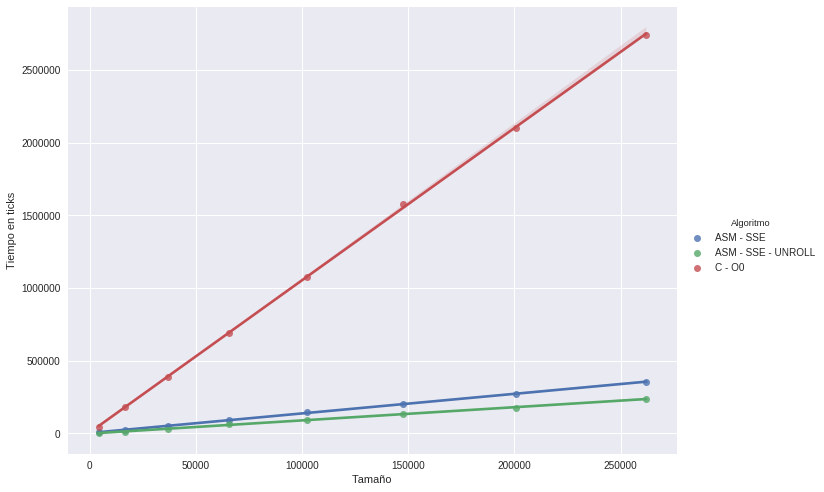
\includegraphics[scale=0.5]{img/fourCombine_UnrollvsNormal.png}
\caption{Versión Unroll del algoritmo puesta en comparación del entregado como respuesta del tp}
\label{sec:unroolvsnormal}
\end{figure}

\begin{figure}[H]
\centering
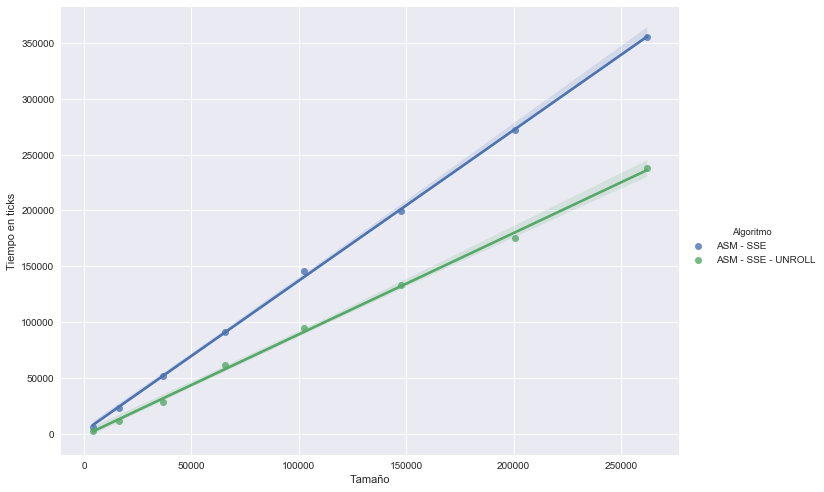
\includegraphics[scale=0.5]{img/fourCombine_UnrollvsNormal_asmOnly.png}
\caption{Comparación exclusiva de las implementaciones en ASM}
\label{sec:unroolvsnormal_asmOnly}
\end{figure}

\begin{figure}[H]
\centering
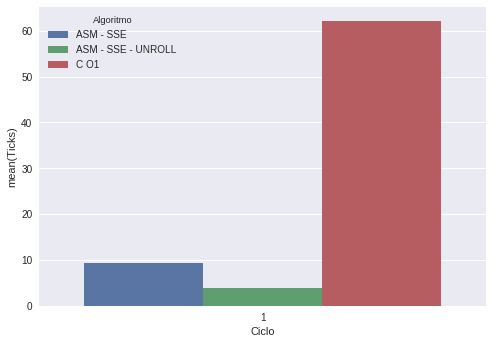
\includegraphics[scale=0.5]{img/fourCombine_ticks_en_ciclo.png}
\caption{Ticks en un ciclo comparación de las 3 implementaciones}
\label{sec:ticksciclo}
\end{figure}

\subsubsection*{Explicación e interpretación de los resultados obtenidos}
Podemos distinguir de la figura 3 que hay una mejora a medida que la imagen se va haciendo cada vez mas grande en el algoritmo de desarrollo del ciclo, esto nos estaría indicando a simple vista que el método funciona, podríamos tener alguna desventaja ya que nuestro programa estaría pesando mas de lo normal, pero esto no sería algo que tenga importancia en un programa como el desarrollado. También se puede hablar de la comparación en imágenes chicas viendo la figura 4. En este caso se trabajo con los resultados mas chicos del set de resultados para poder ver que tan distintos o iguales eran los algoritmos y se puede notar que en imágenes chicas no hay casi diferencia de performance, esto tiene sentido pensando que en imágenes chicas no existe una cantidad de saltos que pueda llegar a influir en la predicción de saltos del procesador.

Por ultimo una manera interesante de ver la diferencia de la performance que se nos ocurrió fue la de medir un ciclo de cada algoritmo y ver que tan performante era cada uno luego de hacer la modificación a esto como se indica en la sección de "como y que van a medir" se puede observar otra manera como la implementación de UNROLL lograr obtener un tiempo que es al menos dos veces mejor que el método puesto en nuestro TP. Este resultado parece contradecir los anteriores dos ya que en estos no se observa que los resultados del UNROLL sean dos veces mejores. No fue testeado pero mi hipótesis recae a que el trabajo que se debe hacer cada vez que se cambia de fila es mayor cuando estamos haciendo el UNROLL , tal vez por la misma ineficiencia de la implementación. Pero este resultado nos muestra el potencial que tiene el UNROLL al poder tener un mejor tiempo de procesamiento por píxel.

Por ultimo voy a hablar de mi test sobre la cache sobre el cual solo quedan los resultados y no hay gráfico asociado . Temo que la  hipótesis que teníamos no se pudo probar ya que los mejores tiempo tanto para el código ASM original como para el ASM - UNROLL son los siguientes :  $243442734$ ticks y $220905687$ ticks respectivamente , hay una mejora de al menos $10\%$ en promedio , cuando se esperaba que al poder leer por filas en nuestro ASM original se podría conseguir una hit rate mas grande. 
\subsection{Conclusiones}
En conclusión el unroll aplicado al algoritmo original logro aumentar la performance mas denotada en imágenes mas grandes. El poder procesar mas píxeles hace que el ciclo sea mas corto y por lo tanto es ahí donde gana tiempo. El algoritmo se podría mejorar para evitar perder tanto tiempo cuando se cambia de fila.

\subsubsection*{Relación entre las hipótesis de trabajo y resultados}